\documentclass[12pt]{article}
 
\usepackage[margin=1in]{geometry} 
\usepackage{graphicx}
\usepackage{url}
\usepackage{hyperref}
\usepackage{float}
\usepackage{quoting}

\usepackage{baskervald}
 
\begin{document}
 
\title{Stargazer Xeru}
\date{}

\maketitle
\begin{figure}[!htb]
  \centering
  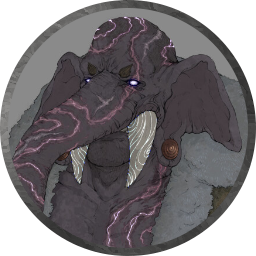
\includegraphics[width=.7\textwidth]{./resources/Stargazer_Xeru}
  \caption{Stargazer Xeru's current appearance.}
\end{figure}

\clearpage

\section{Character Description}

As a Loxodon, Xeru would be a unique visual no matter where he went, but the
angry purple scars that layer his entire body ensure he's remembered where he
passes. At a prodigous 362 years old, Xeru sports large droopy ears, faded skin
and tusks, although the tusks themselves are engraved with some sort of
intricate tribal markings, mirroring his scars. But most people have to look up
to see them, as he stands a striking 8' tall. Given his size, most of his
clothes have to be tailor made, which combined with his unfortutely empty coin
purse, results in him having the one open chested fur cloak, which he always
wears. The cloak is well-made and maintained, dyed a pale green and upon close
inspection has chain-mail hidden underneath. This is mostly redundant, as his
leathery hide turns equally many blows away.

None of this is quite as striking as the halberd he holds; as tall as he is,
blade curved cruelly, Xeru can look quite menacing to the casual observer.
However, those who would speak to him would find him well-mannered and friendly,
especially when sharing a drink... which he does a lot. Xeru unfortunately has
a bit of a drinking problem, which explains where all his gold seems to
dissapear to when you think about how much alcohol it would take to get a 8'
half-ton elephant drunk. Luckily, Xeru comes prepared, hauling many kegs of ale
around with him on his travels, brews he favored across the lands. He only
shares those ales with those he considers family, which for now is his four
party members.

\section{Backstory}

\subsection{The Kerun Clan}

\subsection{A Desperate Doctor}

\subsection{Betrayal}

\section{Related NPCs}

\end{document}
